% Sources: Neso videos (steganography, LSB steganography demo, abstract algebra & number theory intro, prime numbers;
% notes6.md), Stallings 2.5 (steganography). Numbers checked by script (scratchpad/r3/verify3.py).
\definecolor{puregreen}{RGB}{0,255,0}
\definecolor{modgreen}{RGB}{0,252,0}

\section{Steganography}\label{sec:stego}
Encryption hides the \emph{meaning} of a message but not the fact that a secret message is being sent. Ciphertext looks like random gibberish, so it draws attention: an observer immediately knows that something is worth intercepting, may block it, or may pressure the sender and receiver for the key. \textbf{Steganography} (Greek ``covered writing'') solves a different problem. It \textbf{conceals the existence of the message} by hiding it inside an innocent-looking \textbf{cover} such as a text, an image or an audio file, so that an observer does not suspect that any secret communication is taking place. It is \textbf{not an encryption scheme}: the message is not transformed into something unintelligible but merely hidden, and its protection lies in going unnoticed. \textbf{Cryptography}, by contrast, renders the message unintelligible to outsiders by various transformations of the text.

\imp{Cryptography hides the meaning of a message; steganography hides its existence.}
\begin{center}\small
\begin{tabularx}{\textwidth}{@{}l X X@{}}
\toprule
 & \textbf{Cryptography} & \textbf{Steganography}\\
\midrule
Hides & the \textbf{meaning} & the \textbf{existence}\\
Attacker sees & a scrambled message; knows something secret is being sent & an ordinary-looking text/image; doesn't suspect anything\\
Output & ciphertext & a normal-looking \textbf{cover} (text, image, audio) with the message inside\\
\bottomrule
\end{tabularx}
\end{center}
Steganography is the other kind of ``security-related transformation'' $T$ in the model for network security (\S\ref{sec:netmodel}): the transformation applied to the message before transmission does not have to be encryption.

\textbf{Examples from the lecture.} The simplest text steganography arranges words so that some of their letters spell the real message, here the first letter of each word (an \emph{acrostic}, or null cipher). The cover sentence reads as ordinary if odd text, and the secret is the rule ``read the first letters'':
\begin{itemize}
  \item \textbf{S}imply \textbf{e}ncrypt \textbf{c}orrect \textbf{r}eading \textbf{e}xactly \textbf{t}wice. $\Rightarrow$ \textbf{Secret}
  \item \textbf{T}ell \textbf{h}enry \textbf{a}lice \textbf{n}ot \textbf{k}ane / \textbf{Y}esterday \textbf{o}urplan \textbf{u}ndone! $\Rightarrow$ \textbf{Thank You}
\end{itemize}

\subsection{Historical techniques}
Before computers, messages were hidden physically in ordinary documents. Stallings lists four classical techniques; each leaves the document readable as normal text and reveals the hidden marks only under a special treatment that an inspector would not think of applying.
\begin{center}\small
\begin{tabularx}{\textwidth}{@{}l X@{}}
\toprule
Character marking & Chosen letters of a printed or typewritten text are overwritten faintly in pencil. The marks are not visible unless the paper is held at an angle to bright light.\\
Invisible ink & Written with a substance (e.g.\ lemon juice) that leaves no visible trace until heat or a chemical is applied.\\
Pin punctures & Tiny pin holes on selected letters. They are not visible unless the paper is held up in front of a light.\\
Typewriter correction ribbon & Text typed between the lines with a correction ribbon. It is visible only under a strong light.\\
\bottomrule
\end{tabularx}
\end{center}
Modern steganography hides data in digital media instead. Stallings' example is a high-resolution photograph (Kodak Photo CD, $2048 \times 3072$ pixels of 24 bits): changing only the least significant bit of each colour byte does not visibly affect the picture, yet hides $2048 \times 3072 \times 3 = 18\,874\,368$ bits, about 2.3 MB, in a single snapshot. This LSB method is explained below.

\subsection{Drawbacks}
Compared with encryption, steganography has two drawbacks.
\begin{enumerate}[leftmargin=1.5em]
  \item \textbf{Lots of overhead.} A large cover is needed to hide relatively few bits of message: a whole sentence for six letters in the acrostic above, a whole image for a few kilobytes.
  \item \textbf{Once the system is discovered, it becomes virtually worthless.} The security rests entirely on the method staying unknown, which contradicts Kerckhoff's principle (\S\ref{sec:attacks}). Unlike encryption, there is no secret key left to protect the message once the method is known. This can be softened by making the insertion depend on a key (for example, a key that selects which pixels carry the bits).
\end{enumerate}
\textbf{Advantage.} Steganography can be used by parties who have something to lose if the \emph{fact} of their secret communication (not necessarily its content) is discovered. Encryption flags the traffic as important or secret, and may mark the sender or receiver as someone with something to hide; a stego image is just a photograph.

\textbf{Best of both.} A message can be \textbf{first encrypted and then hidden} using steganography. The hiding conceals that communication is taking place, and if the hiding is discovered the attacker still only has ciphertext, which is protected by the key. Encrypted data also looks random, like the noise in the least significant bits it replaces, which makes the hidden data harder to detect statistically.
\begin{center}
\begin{tikzpicture}[node distance=6mm]
  \node[box,fill=cyan!10] (p) {Plaintext};
  \node[box,fill=green!15,right=of p] (e) {Encrypt\\(key)};
  \node[box,fill=yellow!20,right=of e] (c) {Ciphertext};
  \node[box,fill=orange!15,right=of c] (h) {Hide in\\cover};
  \node[box,fill=gray!15,above=4mm of h] (cv) {Cover image};
  \node[box,fill=magenta!8,right=of h] (s) {Stego image\\(looks normal)};
  \draw[arr] (p)--(e); \draw[arr] (e)--(c); \draw[arr] (c)--(h); \draw[arr] (cv)--(h); \draw[arr] (h)--(s);
\end{tikzpicture}
\end{center}

\subsection{LSB steganography}
A byte $b_7 b_6 \dots b_1 b_0$ has the value $128 b_7 + 64 b_6 + \dots + 2 b_1 + b_0$. The leftmost bits are the \textbf{most significant bits} (MSB), because changing them changes the value a lot; the rightmost bits are the \textbf{least significant bits} (LSB), which change it the least:
\[
1010\,10\underbrace{01}_{\text{LSBs}} \qquad\text{bit weights: } 128\;64\;32\;16\;8\;4\;\underline{2\;1}
\]
Changing the lowest $k$ bits of a byte changes its value by at most $2^k - 1$. For $k = 2$ that is at most 3 out of 255, about 1.2\% of the range, which the eye cannot see in a colour.

\textbf{RGB model.} In a 24-bit colour image each pixel is stored as three bytes, one each for the intensity of \textbf{Red}, \textbf{Green} and \textbf{Blue} (0--255).
\begin{center}\small Red $(255,0,0) = (\ttx{11111111}, \ttx{00000000}, \ttx{00000000})$ \quad Green $(0,255,0)$ \quad Blue $(0,0,255)$\end{center}

\begin{center}
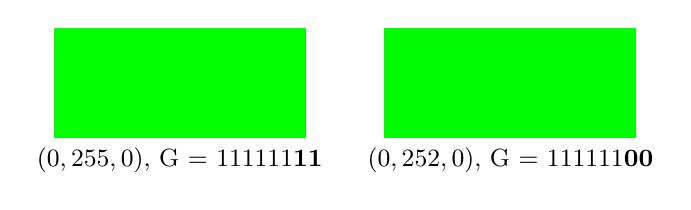
\begin{tikzpicture}
  \fill[puregreen] (0,0) rectangle (3.2,1.4);
  \fill[modgreen] (4.2,0) rectangle (7.4,1.4);
  \node[font=\small,below] at (1.6,0) {$(0, 255, 0)$, G $=$ \ttx{111111\textbf{11}}};
  \node[font=\small,below] at (5.8,0) {$(0, 252, 0)$, G $=$ \ttx{111111\textbf{00}}};
\end{tikzpicture}
\end{center}
The two boxes look identical, but the last 2 bits of their green values differ. \textbf{Those LSBs can therefore store hidden information}: the sender overwrites them with message bits, and the image looks unchanged. Using the 2 LSBs of each of R, G and B hides $2 \times 3 = \mathbf{6}$ \textbf{bits per pixel}, and no channel value changes by more than 3. To extract the message the receiver simply reads the last 2 bits of each channel, in the agreed order of pixels, and concatenates them.

\begin{worked}[: hiding bits in one pixel]
\textbf{Q.} Hide the six bits \ttx{11 01 10} in the pixel $(100, 50, 200)$ using the 2 LSBs of each channel. By how much does each value change?

Write each value in binary and replace its last two bits with the next two message bits:
\begin{center}\small
\begin{tabular}{@{}lllll@{}}
\toprule
Channel & Value & Binary & Replace last 2 bits & New value\\
\midrule
R & 100 & \ttx{011001\textbf{00}} & \ttx{011001\textbf{11}} & 103 ($+3$)\\
G & 50 & \ttx{001100\textbf{10}} & \ttx{001100\textbf{01}} & 49 ($-1$)\\
B & 200 & \ttx{110010\textbf{00}} & \ttx{110010\textbf{10}} & 202 ($+2$)\\
\bottomrule
\end{tabular}
\end{center}
New pixel \textbf{(103, 49, 202)}; every channel changes by at most 3, as predicted. Check: the last two bits of 103, 49, 202 are \ttx{11}, \ttx{01}, \ttx{10} \checkmark.
\end{worked}

\textbf{Capacity.} With 6 bits per pixel an $800 \times 600$ image holds $800 \cdot 600 \cdot 6 = 2{,}880{,}000$ bits $= 360{,}000$ bytes. With only the single LSB of each channel (3 bits per pixel) a $1024 \times 768$ image holds $1024 \cdot 768 \cdot 3 = 2{,}359{,}296$ bits $= 294{,}912$ bytes. The lecture's 17-byte message ``Kill Corona Virus'' is $17 \times 8 = 136$ bits, which needs only $\lceil 136 / 6 \rceil = 23$ pixels at 6 bits per pixel.

\textbf{Blue orchids:} the lecture shows the image without and with hidden information side by side, and they cannot be told apart.

\textbf{Detection.} Looking at the image reveals nothing, but a statistical analysis may. In a natural photograph the LSBs are correlated with the rest of the image, while embedded data (especially encrypted data) is uniformly random, so the LSB plane of a stego image has slightly different statistics; a changed file format or file size is a further clue (see the OpenStego demo below). The study of detecting hidden data is called \textbf{steganalysis}.

\subsection{Watermarking vs.\ image steganography}
Both techniques embed extra information in an image, but for opposite purposes. A \textbf{watermark} is embedded to \textbf{prove ownership} or copyright: the logo or owner information is not secret, it is often visible (like the \ttx{nesoacademy.org} mark on the lecture's laptop image), and it must survive cropping and compression so that it can still be shown later. \textbf{Image steganography} embeds a message for \textbf{secret communication}: its \textbf{existence} must stay hidden, and robustness matters less than going unnoticed.
\begin{center}\small
\begin{tabularx}{\textwidth}{@{}l X X@{}}
\toprule
 & \textbf{Watermarking} & \textbf{Image steganography}\\
\midrule
Purpose & prove \textbf{ownership} / copyright & \textbf{secret communication}\\
Is the mark secret? & no; it's often visible (like the \ttx{nesoacademy.org} logo) & yes; its \textbf{existence} is hidden\\
Hidden data & logo, owner info & any message or file\\
\bottomrule
\end{tabularx}
\end{center}

\subsection{OpenStego demo}
OpenStego is a free tool that embeds a file in an image and extracts it again. The lecture uses it in both directions:
\begin{enumerate}[leftmargin=1.5em]
  \item \textbf{Hide Data:} message file \ttx{My Message.txt} (``Kill Corona Virus'', 17 bytes) + cover file \ttx{Blue Orchids.jpg} (58.4 KB) $\to$ stego file \ttx{BO.png} (824 KB). No password. ``Message embedded into 1 cover file(s).''
  \item \textbf{Extract Data:} input \ttx{BO.png} $\to$ output folder. ``Message file extracted successfully'', and the text file comes back unchanged.
\end{enumerate}
\textbf{Why PNG, and why so much bigger} (not explained in the video): JPEG compression is lossy, so it slightly changes pixel values when the image is saved, which would wipe out the hidden LSBs. The stego image is therefore saved in the lossless PNG format, which stores every pixel exactly and is much larger (58.4 KB $\to$ 824 KB). That size jump is itself a hint that something is going on. Leaving the password empty means the extraction needs no key, so anyone who suspects the file and has the tool can read the message; with a password OpenStego encrypts the data before hiding it, which is the encrypt-then-hide combination above.

\section{Prime Numbers}\label{sec:primesintro}
\textbf{Why the course turns to mathematics.} Classical ciphers substitute and move letters. Modern cryptography treats plaintext and ciphertext as \emph{numbers}, and most encryption is based heavily on \textbf{number theory} and \textbf{abstract algebra}; calculus and trigonometry make no major contribution. The concepts needed are the division and Euclidean algorithms and the extended Euclidean algorithm (\S\ref{sec:exteuclid}), modular arithmetic (\S\ref{sec:modular}), groups, rings, fields and finite fields with polynomial arithmetic (\S\ref{sec:algebra}), Euler's totient (\S\ref{sec:totient}), Fermat's and Euler's theorems (\S\ref{sec:fermat}), and primality testing, the Chinese remainder theorem and discrete logarithms (\S\ref{sec:primes}). The lecture also notes that this is cryptography for classical computers; quantum computers will need different assumptions, because a quantum algorithm (Shor's) factors efficiently. Primes come first because almost everything else is built on them.

\textbf{Definitions.} A \textbf{prime} is an integer greater than 1 with exactly two divisors, 1 and itself: it cannot be divided by any other number without leaving a remainder. A \textbf{composite} number has more than two divisors. \textbf{1 is neither}, because it has only one divisor. Examples: 2, 3, 5, 7 are prime; $9 = 3^2$ (divisors 1, 3, 9) and $33 = 3 \cdot 11$ (divisors 1, 3, 11, 33) are composite.

\textbf{Facts.} 2 is the smallest prime and the \textbf{only even prime}, since every larger even number has 2 as a third divisor. Except for 2 and 5, every prime ends in the digit 1, 3, 7 or 9: a number ending in 0, 2, 4, 6 or 8 is divisible by 2, and one ending in 5 is divisible by 5. (The converse fails: $33$ and $39$ end in 3 and 9 but are composite.)

\textbf{Every number has prime factors.} By the \textbf{fundamental theorem of arithmetic}, every integer $n > 1$ can be written as a product of primes in exactly one way, apart from the order of the factors. A prime is its own factorisation; 1 is not a factor to be listed, since it is not prime.
\begin{center}\small
\begin{tabular}{@{}rl@{\qquad}rl@{}}
\toprule
$n$ & factorisation & $n$ & factorisation\\
\midrule
10 & $2 \cdot 5$ & 37 & $37$ (prime)\\
11 & $11$ (prime) & 308 & $2^2 \cdot 7 \cdot 11$\\
100 & $2^2 \cdot 5^2$ (9 divisors) & 14688 & $2^5 \cdot 3^3 \cdot 17$\\
\bottomrule
\end{tabular}
\end{center}
The number of divisors follows from the factorisation: a divisor of $2^2 \cdot 5^2$ is $2^a 5^b$ with $a, b \in \{0, 1, 2\}$, giving $3 \times 3 = 9$ divisors of 100 (1, 2, 4, 5, 10, 20, 25, 50, 100).

\subsection{Why primes matter in cryptography}
Many encryption algorithms, RSA first among them (\S\ref{sec:rsa}), are based on prime numbers, because of an asymmetry in the work involved. \textbf{Multiplying} two large primes is \textbf{very fast}: two 300-digit numbers are multiplied in a fraction of a millisecond. The \textbf{reverse}, \textbf{factoring} the product back into its primes, is \textbf{extremely computer-intensive}: no known classical algorithm does it in polynomial time, and for a product of two well-chosen 1024-bit primes all the computers in the world would take far too long (\S\ref{sec:primes} covers the factoring methods).
\[
p, q \;\xrightarrow{\text{easy}}\; n = p \cdot q \qquad\qquad n \;\xrightarrow{\text{very hard}}\; p, q
\]
A function that is easy to compute but infeasible to reverse is called a \textbf{one-way function}; if a secret (here the primes $p$ and $q$) makes the reverse easy, it is a \textbf{trapdoor one-way function}, which is exactly what a public-key cipher needs. Cryptographic algorithms therefore use \textbf{large} primes, hundreds of digits long. The lecture closes with six numbers to test, from 4 to 34 digits: 5393, 27644437, 4398042316799, 1125899839733759, 18014398241046527 and 1298074214633706835075030044377087. \textbf{All six are prime} (checked with the Miller--Rabin test of \S\ref{sec:primes}); trial division would need about $\sqrt{n}$ steps, which is hopeless for the last one, and this is why fast probabilistic primality tests matter.

\begin{mustknow}[: primes]
Prime: $> 1$ with exactly two divisors (1 and itself); 1 is not prime; 2 is the only even prime. Every $n > 1$ factors uniquely into primes, e.g.\ $14688 = 2^5 \cdot 3^3 \cdot 17$.\\
Security of RSA-type systems rests on \textbf{factoring the product} $n = pq$ of two large primes being infeasible, while multiplying $p$ and $q$ is easy.
\end{mustknow}

\begin{fixbox}
\begin{itemize}
  \item \textbf{Slide wording:} ``Factoring very large prime numbers is very hard'' should say factoring the \emph{product} of two large primes. A prime can't be factored at all.
  \item The factorisation table writes $11 = 1^1 \times 11^1$ and lists 1 as a prime factor. 1 is not prime; 11 and 37 are simply prime.
  \item The notes call watermarks ``typically visible''. The lecture's example is visible, but watermarks can also be invisible. The real difference is the purpose (ownership vs.\ secret communication).
  \item Fermat's and Euler's theorems need $\gcd(a,p) = 1$ / $\gcd(a,n) = 1$; the notes omitted this condition.
  \item Everything else checked: TOMATO $\to$ (a) (by script), $N(N-1)/2$, all six numbers prime, factorisations correct.
\end{itemize}
\end{fixbox}
